\chapter{Entwicklung der Schaltung}
Dieses Kapitel beschreibt die Entwicklung der Schaltung.
Es werden die verschiedenen Schaltungstopologien in Simulationen 
verglichen und eine Schaltung ausgewählt.
Weiterhin wird für die gewählte Schaltung ein PCB entwickelt und dieses dann
bestückt.

\section{Vergleich der Schaltungstopologien}
\subsection{Nutzung einer integrierten Schaltung}
Aufgrund der hohen notwendigen Versorgungsspannung ist die Auswahl möglicher 
Spannungsregler klein.

Vom Hersteller Texas Instruments ist im Bereich der „Ultra Low Noise“ 
Linearregler nur ein Modell verfügbar.
Der LP38798 hat einen Ausgangsspannungsbereich von 0\,\si{\volt} bis
20\,\si{\volt}, einen maximalen Ausgangsstrom von 800\,\si{\milli\volt} und
ein Ausgangsrauschen von 5\,$\si{\micro\volt}_{\rm rms}$

\subsection{Nutzung einer Operationsverstärkerschaltung}
Eine Alternative zur integrierten Schaltung ist die Nutzung eines 
Transistors als steuerbaren Widerstand und die Ansteuerung des Transistors
mit einem Operationsverstärker.
Die Abb.:~\ref{FIG:LINREG} aus dem vorherigen Kapitel beschreibt eine solche 
Schaltung.

Die Eigenschaften des Operationsverstärkers sollten neben einer hohen 
Leerlaufverstärkung, eine hohe hohe Unempfindlichkeit gegen 
Versorgungsspannungsänderungen und ein geringes Rauschen am Ausgang sein.

Die Spannungsreferenz selber sollte möglichst rauscharm und Temperaturstabil 
sein.
Für diese Anwendung lassen sich Z-Dioden nutzen, diese erzeugen allerdings 
besonders ab 5\,V, da hier der Lavinendurchbruch dominiert ein ausgeprägtes
Schrotrauschen. Die Nutzung einer kleineren Diode erfordert einen 
Spannungsteiler im Feedbackpfad, der selber wieder ein Rauschen erzeugt.
An der Diode entstandenes Rauschen kann durch eine entsprechende 
Filterschaltung begrenzt werden.

Der Transistor sollte den Ausgangsstrom führen können und die Verlustleistung
abführen können.
Da MOSFET Typen ein ausgeprägtes 1/f-Rauschen erzeugen sind an dieser 
Stelle nur Bipolartransistoren oder JFET eine Option.

\subsection{Nutzung einer diskreten Transistorschaltung}
\begin{figure}
  \centering
  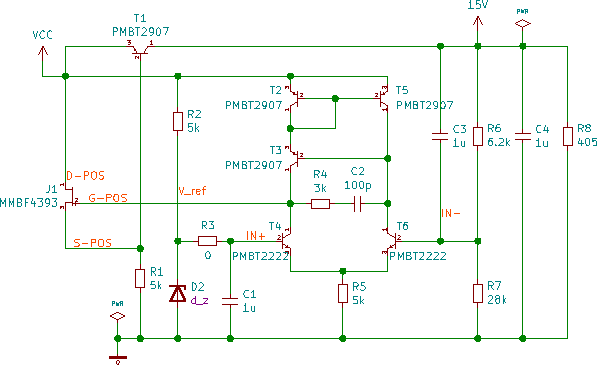
\includegraphics[clip, width=0.80\textwidth]{./../common/schaltungen/reg.pdf}
  \caption{Linearregler}\label{FIG:REG}
\end{figure}
Eine weitere Alternative ist die Nutzung einer diskreten Transistorschaltung
Hierbei wird ein diskret aufgebauter Operationsverstärker aufgebaut um
die Ausgangsspannung auf den Sollwert zu regeln.
Ein diskret aufgebauter Operationsverstärker ermöglicht es weiterhin Rauschen
an beliebigen Stellen durch Filterschaltungen zu unterdrücken.

Die Abb.:~\ref{FIG:REG} zeigt einen Schaltungsvorschlag.
Die Schaltung selber besteht aus einem Differenzverstärker bestehend aus einem
Wilson Stromspiegel und zwei NPN Transistoren und einem JFET-PNP 
Ausgangstreiber.
Die Spannungsreferenz wird über eine Z-Diode und einem RC-Tiefpass erzeugt.
Die Ausgangsspannung wird mittels Spannungsteiler auf die Referenzspannung 
heruntergeteilt, so dass die Ausgangsspannung der Sollspannung entspricht.
 
\section{Auswahl der Schaltung}
Zur Auswahl der Schaltung wurden alle Schaltungsvorschläge mittels 
SPICE-Simulation simuliert. Die Ergebnisse sind in den Abbildungen [TODO] 
aufgeführt.
Die Abbildungen zeigen die Rauchleistung am Ausgang der jeweiligen Schaltung.

\section{Entwicklung und Bestückung des PCB}
\begin{figure}
  \centering
  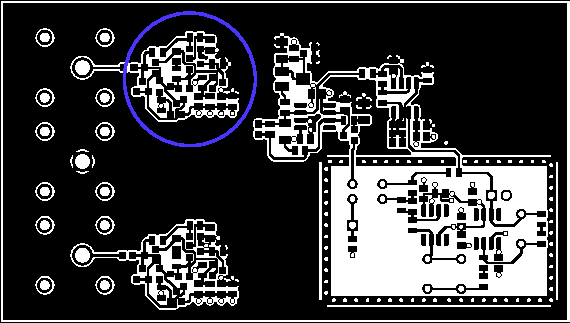
\includegraphics[clip, width=0.49\textwidth]{./../common/bilder/pcb-wien.pdf}
  \caption{Wien-Brücke mit Spannungsversorgung}\label{FIG:PCB}
\end{figure}
Nach der Auswahl der Schaltung wurde ein PCB erstellt und bestückt.
Die Abbildung~\ref{FIG:PCB} zeigt das PCB der Schaltung zusammen mit der Last.
Der Positivspannungsregler wurde blau markiert.
Die einzelnen Schaltungsbestandteile wurden als Gruppe auf der Schaltung 
platziert und können bei Bedarf auch überbrückt werden. So ist es möglich auch
bei einem Fehler in einer Schaltung, die restlichen Bestandteile 
weiterzubetreiben. 
